\documentclass[a4paper,10pt,twocolumn,uplatex,dvipdfmx]{jsarticle}

\usepackage{amsmath}
\usepackage{array}
\usepackage{booktabs}
\usepackage{graphicx}
\usepackage[alphabet]{pxchfon}
\usepackage{tabularx}
\usepackage{pdflscape}
\usepackage{capt-of}
\usepackage{xcolor}
\usepackage{url}

\setlength{\columnsep}{8mm}
\setlength{\parindent}{1zw}
\setlength{\parskip}{0.15\baselineskip}
\renewcommand{\arraystretch}{1.22}
\urlstyle{same}

\definecolor{deepblue}{RGB}{36,79,121}
\definecolor{softgray}{RGB}{245,246,247}
\definecolor{unknown}{RGB}{140,40,40}

\newcolumntype{Y}{>{\raggedright\arraybackslash}X}
\newcommand{\unknownmark}{\textcolor{unknown}{\textbf{?}}}
\newcommand{\species}[1]{\textit{#1}}
\newcommand{\Tpeak}{$T_{\mathrm{peak}}$}
\newcommand{\dTpeak}{$\Delta T_{\mathrm{peak}}$}

\title{\textbf{修士研究中間報告\\
マカク RGC 応答を用いた生理制約付き Retina SNN の\\
動的有効受容野同定}}
\author{M1 TANG YU}
\date{2026年7月31日}

\begin{document}

\maketitle

\begin{abstract}
本研究は、霊長類網膜の回路構造と生理的範囲を明示的な制約として用い、
直接測定が不足する低次元パラメータをマカク記録 RGC 応答から学習する
動的有効受容野モデリング手法を提案する。錐体、H1 水平細胞、
ON/OFF 双極細胞、局所アマクリン細胞、ON/OFF RGC を
解釈可能な処理段として構成し、接続方向、極性、局所性、細胞型を固定する。
RGC は膜電位、適応状態、発火閾値を持つ spiking unit として表現し、
記録 spike を教師信号として学習する。
結合強度、時定数、抑制動態、適応特性は生理的範囲内で学習し、
RF は学習後の RGC 応答から推定する。主評価にはマカク記録データを用い、
ヒト設定は独立した転移プロファイルとして扱う。細胞間接続、
既知・未知の生理データ、パラメータ決定方針、学習手順、
実験上のリスクと対照条件を一体として整理する。
\end{abstract}


\section{研究目的と提案手法の位置づけ}

\subsection{研究目的}

本研究の目的は、既知の霊長類網膜回路と生理的パラメータ範囲を
モデル内部へ組み込み、RGC の動的有効受容野を記録応答から同定できる
生理制約付きグレーボックス SNN を構築することである。
入力段では ISETBio により光学像と錐体励起を生成し
\cite{brainard2015}、水平細胞、双極細胞、アマクリン細胞、RGC の
各処理段を明示する。

本報告でいう動的有効受容野とは、モデルへ直接与える固定 RF
カーネルではなく、学習後に凍結したモデルの応答に対して
STA、刺激摂動、Jacobian などから推定する、時間、内部状態、
刺激条件に依存する入力感度である。

\noindent\textbf{研究課題：}
マカク RGC 記録応答に対し、回路構造を固定し、低次元の
生理パラメータのみを学習することで、無制約モデルに近い予測性能を
維持しながら、再現性の高い動的有効受容野を得られるか。

受容野を記述する LN/GLM と point-process model は、
刺激フィルタ、発火履歴、細胞間結合を解釈可能な形で推定できる
\cite{pillow2008}。霊長類 midget 経路については、
文献由来の回路・空間パラメータを統合する信号処理モデル
\cite{somaratna2025}、光学・解剖・生理を偏心度ごとに統合する
image-computable RF mosaic
\cite{cottaris2026} が報告されている。本研究はこれらの知見を基盤とし、
明示的な中間細胞、時間動態、スパイク生成、部分学習可能な生理制約、
学習後の dynamic RF 評価を同一の枠組みで扱う。

\subsection{中心仮説}

生理制約は、自由度の高い応答近似と比較して、少数データ条件における
RF の安定性、刺激統計をまたぐ汎化、細胞型ごとの整合性、
回路機構の追跡可能性を高めると仮定する。予測性能、RF の再現性、
学習パラメータの生理範囲、機構消融の結果を組み合わせて検証する。

\subsection{回路として固定する要素}

モデルは次の生理的制約を保持する。

\begin{itemize}
  \item L/M 錐体から H1 水平細胞への入力と、H1 から錐体終末への側方フィードバック
  \item 錐体から ON/OFF 双極細胞への符号反転・符号保存分岐
  \item 双極細胞から RGC への直接興奮性経路
  \item 双極細胞からアマクリン細胞を介する並列抑制経路
  \item ON/OFF RGC と視神経スパイク出力
\end{itemize}

これらはネットワークトポロジーと符号を定める。定量値の扱いは
DATA-FIXED、BIO-FIXED、BOUNDED-LEARNED、
VALIDATION-TUNED、POST-HOC の五区分で管理する。

\section{Spiking Neural Network の基礎}

\subsection{SNN の基本概念}

Artificial Neural Network（ANN）では、各 unit が実数値の activation を
次層へ伝える。これに対して Spiking Neural Network（SNN）では、
各 neuron が内部状態を時間方向に保持し、膜電位が閾値を超えた時刻に
離散的な spike を出力する。したがって、SNN は入力値だけでなく、
入力が到着した時刻、過去の内部状態、直前の発火履歴を計算に含む
動的システムである \cite{maass1997,gerstner2014}。

Spike train は、時間 bin $t$ における発火の有無
$z_i^t\in\{0,1\}$、または bin 内 spike count として表現できる。
情報は平均発火率だけでなく、発火時刻、spike 間隔、複数 neuron 間の
同期・非同期関係にも含まれ得る。どの符号化を採用するかは
課題と測定データによって決める必要がある。

\subsection{Leaky Integrate-and-Fire neuron}

本研究の RGC unit の基本形は、Leaky Integrate-and-Fire（LIF）
neuron である。LIF は詳細な ion channel を逐一再現せず、
入力の積分、膜電位の漏れ、閾値発火、reset という
spike generation の主要機能を低次元状態で表す
\cite{gerstner2014}。

離散時間幅を $\Delta t$、膜時定数を $\tau_{m,i}$、
$\alpha_i=\exp(-\Delta t/\tau_{m,i})$ とすると、neuron $i$ の
基本更新は次のように書ける。

\begin{align}
  \widetilde{v}_i^{t+1}
  &= \alpha_i v_i^t + (1-\alpha_i)I_i^t, \\
  z_i^{t+1}
  &= H(\widetilde{v}_i^{t+1}-\theta_i), \\
  v_i^{t+1}
  &= (1-z_i^{t+1})\widetilde{v}_i^{t+1}
     + z_i^{t+1}v_{\mathrm{reset},i}.
\end{align}

ここで $I_i^t$ は上流入力、$v_i^t$ は膜電位、
$\theta_i$ は発火閾値、$H$ は step function である。
適応型 neuron では、発火後に閾値または抑制状態を増加させ、
時間とともに減衰させることで spike-frequency adaptation を表現する。

\subsection{離散時間の基本アルゴリズム}

\noindent\fcolorbox{deepblue}{softgray}{%
\parbox{\dimexpr\linewidth-2\fboxsep-2\fboxrule\relax}{\small
\textbf{1. 入力：}時刻 $t$ の cone response と上流細胞状態を受け取る。\par
\textbf{2. シナプス統合：}局所接続内の入力を重み付き加算する。\par
\textbf{3. 状態更新：}膜電位、適応、抑制などを一時間 step 更新する。\par
\textbf{4. 発火判定：}膜電位が閾値を超えた neuron から spike を出力する。\par
\textbf{5. Reset：}発火 neuron の膜電位と適応状態を更新する。\par
\textbf{6. 時間展開：}全 stimulus bin について 1--5 を反復する。
}}

この反復により、同じ瞬間入力であっても、それ以前の刺激と発火履歴が
異なれば出力が変化する。これが本研究で扱う dynamic effective RF と
整合する重要な性質である。

\subsection{SNN の学習方法}

SNN の step function は発火点で不連続であり、それ以外では
微分がほぼゼロである。そのため、通常の backpropagation をそのまま
適用すると勾配を伝えられない。Surrogate gradient 法では、
forward 計算では hard spike を使用し、backward 計算だけで
step function の微分を滑らかな近似関数へ置き換える
\cite{neftci2019,eshraghian2023}。

\begin{equation}
  \frac{\partial H(v-\theta)}{\partial v}
  \ \approx\ \phi_{\beta}(v-\theta),
\end{equation}

ここで $\phi_{\beta}$ は sigmoid derivative や三角形関数などの
surrogate derivative である。Network を時間方向へ展開し、
Backpropagation Through Time（BPTT）によって weight、gain、
time constant、threshold などの勾配を計算する。

本研究では、recorded RGC ごとに一つの model output unit を対応させ、
model spike probability または firing rate と recorded spike の
likelihood loss を計算する。Cell type、ON/OFF polarity、
eccentricity、接続 topology、興奮・抑制符号は学習せず固定する。
RF 形状は loss に与えず、学習後に凍結したモデルから
STA、Jacobian、GLM readout により抽出する。

\subsection{ANN と SNN の比較}

\begin{table*}[t]
\centering
\caption{ANN と SNN の基本的な相違、および本研究での意味。}
\label{tab:ann-snn-comparison}
\small
\setlength{\tabcolsep}{4pt}
\begin{tabularx}{0.98\textwidth}{
  >{\raggedright\arraybackslash}p{0.13\textwidth}
  >{\raggedright\arraybackslash}p{0.25\textwidth}
  >{\raggedright\arraybackslash}p{0.27\textwidth}
  Y}
\toprule
\textbf{観点} &
\textbf{ANN} &
\textbf{SNN} &
\textbf{本研究での意味} \\
\midrule

信号表現 &
連続値 activation を層間で伝達する &
離散 spike と発火時刻を伝達する &
記録 RGC spike と model output を直接対応させる \\

時間と状態 &
Feedforward ANN では時間状態を持たず、
RNN では別途 hidden state を定義する &
膜電位、適応、refractory state が neuron 内部に組み込まれる &
刺激履歴と内部状態に依存する応答を明示的に扱う \\

出力 &
分類確率、回帰値、連続 feature が一般的である &
Spike、spike probability、filtered firing rate を出力できる &
Recorded spike likelihood を主学習目標にできる \\

学習 &
連続 activation を通常の backpropagation で学習する
\cite{lecun2015} &
Surrogate gradient、ANN-to-SNN conversion、局所学習則などを用いる
\cite{neftci2019,rueckauer2017} &
Hard spike forward と surrogate-gradient BPTT を用いる \\

計算 &
Dense multiply--accumulate が中心である &
Spike が疎な場合、event-driven accumulate が可能である &
将来の neuromorphic deployment では利点になり得るが、
通常 GPU 上の学習効率を保証しない \\

生理解釈 &
高い近似能力を持つが、unit state と生理量の対応は任意である &
Membrane、threshold、adaptation、synaptic delay を
生理量と対応させやすい &
既知回路を固定し、未測定 dynamics のみを有界学習する \\

\bottomrule
\end{tabularx}
\end{table*}

\subsection{SNN の主な利点}

\begin{itemize}
  \item \textbf{時間情報を直接扱える：}
        発火率だけでなく spike timing と履歴依存性を表現できる。
  \item \textbf{内部状態を保持できる：}
        膜電位、適応、refractory state が短期記憶として働く。
  \item \textbf{観測 spike と出力形式が一致する：}
        RGC spike train を余分な出力変換なしに教師信号として扱える。
  \item \textbf{生理パラメータとの対応を作りやすい：}
        Time constant、threshold、adaptation、synaptic delay を
        model parameter として明示できる。
  \item \textbf{Event-driven 計算へ展開できる：}
        Spike が疎で専用 hardware を利用する場合、不要な演算と通信を
        減らせる可能性がある \cite{roy2019,davies2018}。
\end{itemize}

一方、ANN は学習手法、software、GPU 実装が成熟しており、
多くの静的課題では高速かつ高精度である \cite{lecun2015}。
したがって、SNN の利点は課題、データ、時間分解能、spike sparsity、
hardware に依存し、ANN に対する一般的な優越性を意味しない。

\subsection{SNN を採用する理由}

本研究で SNN を採用する第一の理由は、RGC の実験出力そのものが
spike train だからである。連続値の中間表現から spike を後付けで生成する
構成より、膜電位、閾値、発火履歴、適応を持つ output unit を用いる方が、
観測量と model state の対応を明示しやすい。

第二に、本研究の対象は固定された一枚の RF ではなく、
刺激履歴、contrast、内部状態によって変化する dynamic effective RF である。
SNN は時間状態を内部に保持するため、膜時定数、adaptation、
delayed inhibition が RF の時間変化へどのように寄与したかを
module ablation で追跡できる。

第三に、生理的制約を parameter と topology に直接対応させやすい。
ON/OFF polarity、局所接続、興奮・抑制符号、cell type を固定し、
gain、time constant、adaptation、threshold のみを
生理範囲内で学習することで、完全な black-box fitting と
全固定 mechanistic model の中間に位置する grey-box model を構成できる。

第四に、SNN は sparse spike と event-driven hardware を組み合わせた場合、
計算・通信を event 発生時へ限定できる可能性がある
\cite{roy2019,davies2018}。ただし、これは neuromorphic hardware 上での
実装上の可能性であり、本研究の主目的ではない。通常の GPU 上で
時間展開する SNN が ANN より自動的に高速または低消費電力になるとは
仮定しない。

\subsection{現在の Retina SNN の位置づけ}

現在の実装は、H1、双極細胞、アマクリン細胞に連続値の動的状態を持たせ、
RGC population に membrane、adaptation、hard spike、
spike probability、filtered rate を持たせる hybrid dynamical SNN である。
したがって、全中間細胞が hard spike を出力するという意味での
fully spiking model ではない。網膜では photoreceptor、horizontal cell、
bipolar cell の多くが graded potential を用いるため、この構成は
生理的役割との対応を保ちながら RGC spike output を明示する。

SNN の採用自体を性能向上の根拠とはしない。同一データ split と
likelihood を用いた point-process GLM、同容量 ANN/RNN、
全固定生理モデルとの比較により、spiking state と生理制約が
RF stability、cross-stimulus generalization、少数データ条件に
追加の価値を持つかを検証する。

\section{信号フロー図とデータの構成}

図\ref{fig:retina-flow}は、自然画像から視神経出力までの回路構造を示す。
図\ref{fig:training-evaluation-flow}は、マカク記録 RGC 応答を用いる
学習経路と、モデル凍結後の動的有効受容野の抽出経路を示す。
通常矢印は興奮性入力、
曲線矢印はフィードバック、T 字端は抑制、破線は弱い入力、
二重線はネットワーク結合を表す。

細胞間の収束・発散関係は表\ref{tab:connectivity}に示す。
錐体密度、受容野径、応答時間、測定条件、物種差は
表\ref{tab:physiology}に示す。これにより、回路の接続関係と
定量的な生理根拠を独立して参照できる。

\begin{figure*}[t]
  \centering
  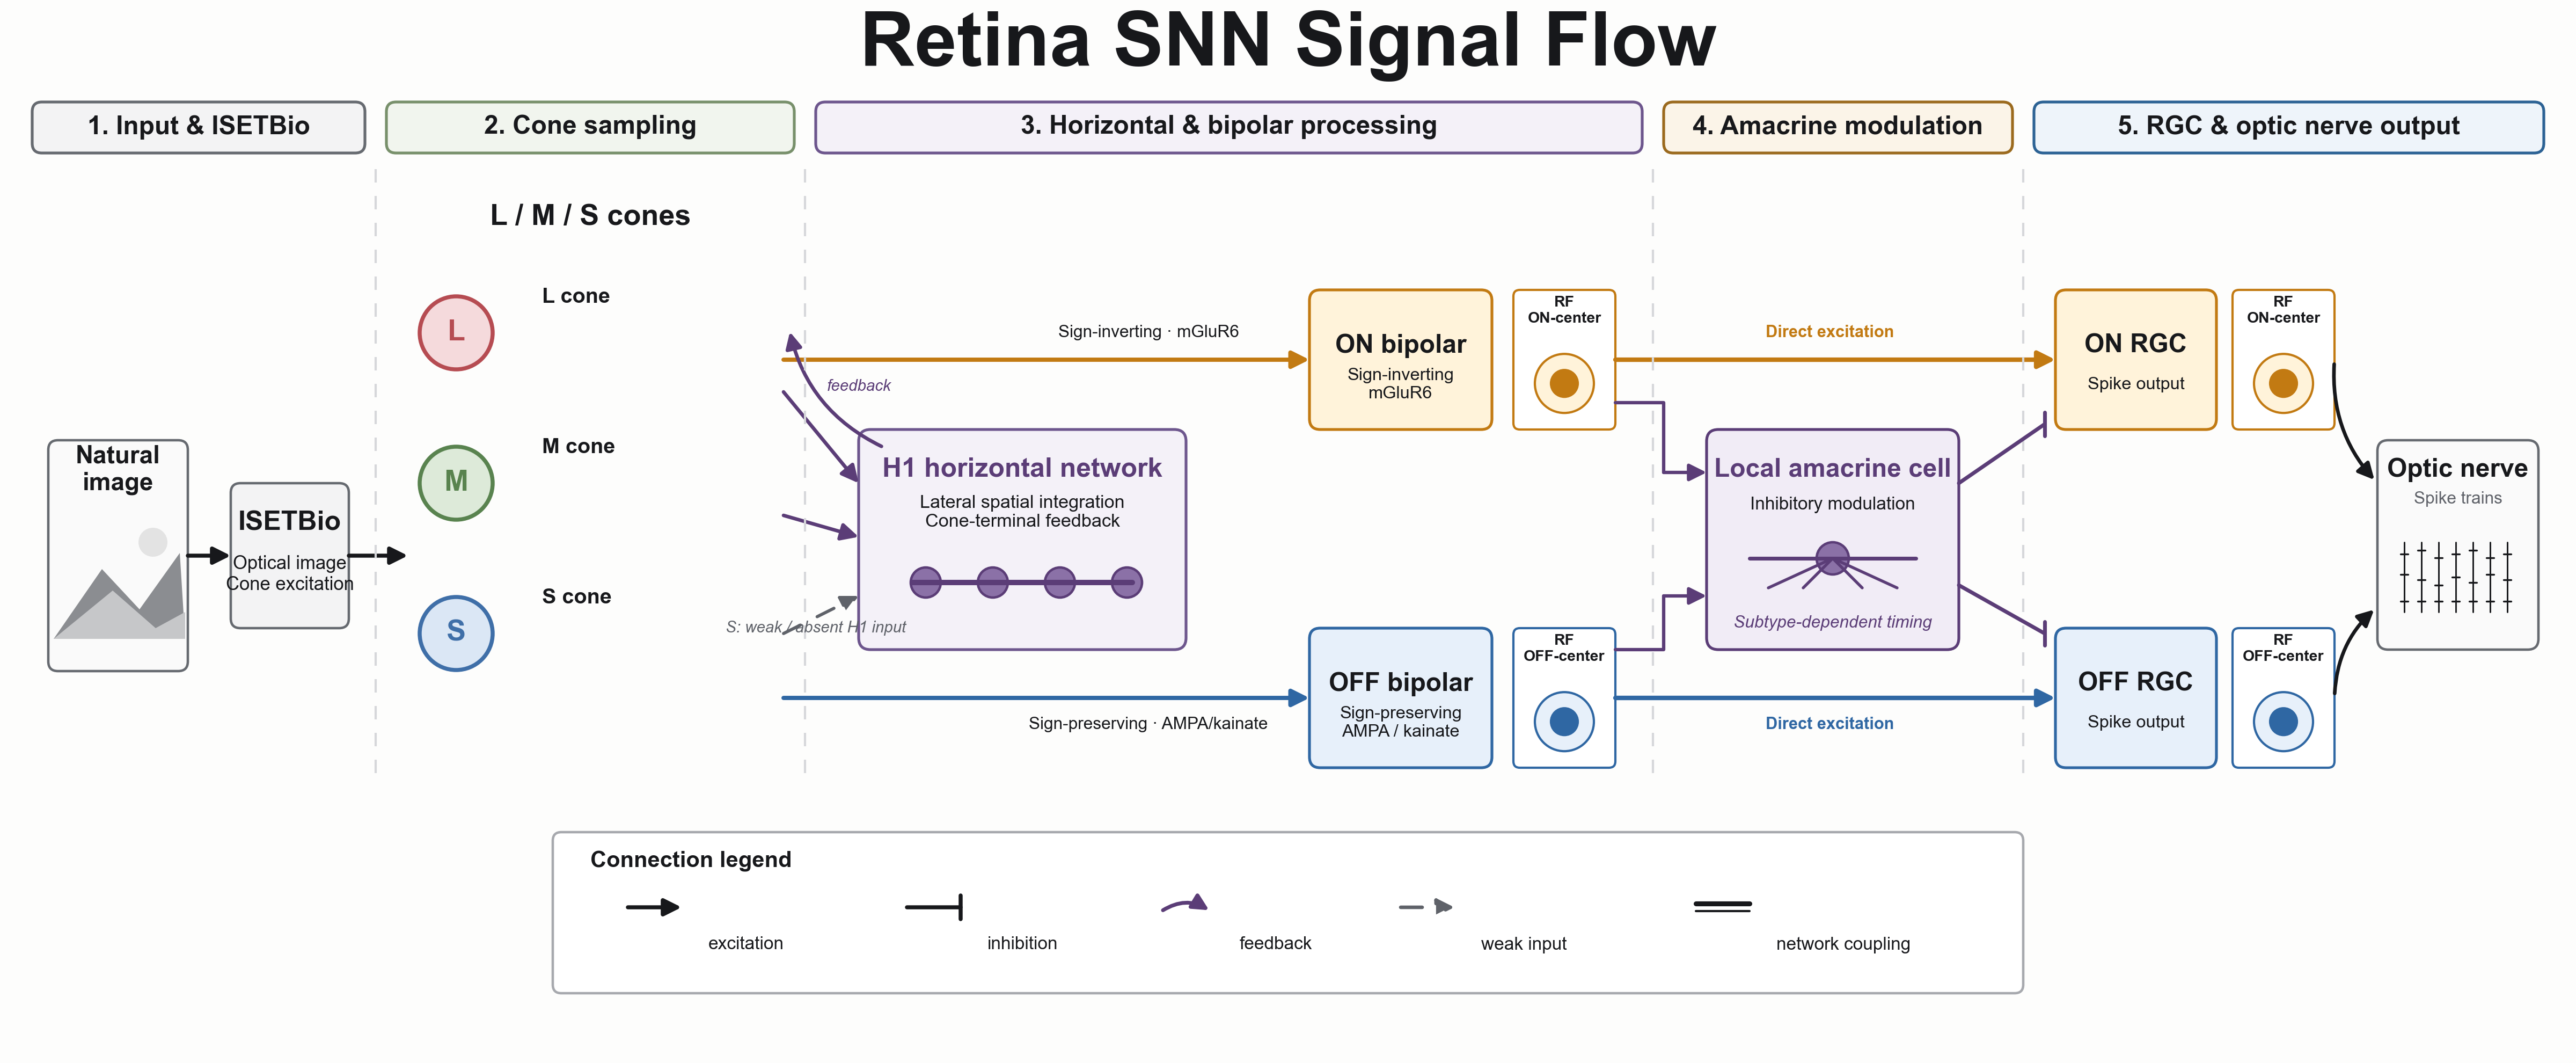
\includegraphics[width=\textwidth]{assets/retina_snn_signal_flow.png}
  \caption{Retina SNN の生理信号フロー。回路構造と接続種別を示す。
  細胞間接続は表\ref{tab:connectivity}、定量的な生理データは
  表\ref{tab:physiology}に示す。}
  \label{fig:retina-flow}
\end{figure*}

\begin{figure*}[t]
  \centering
  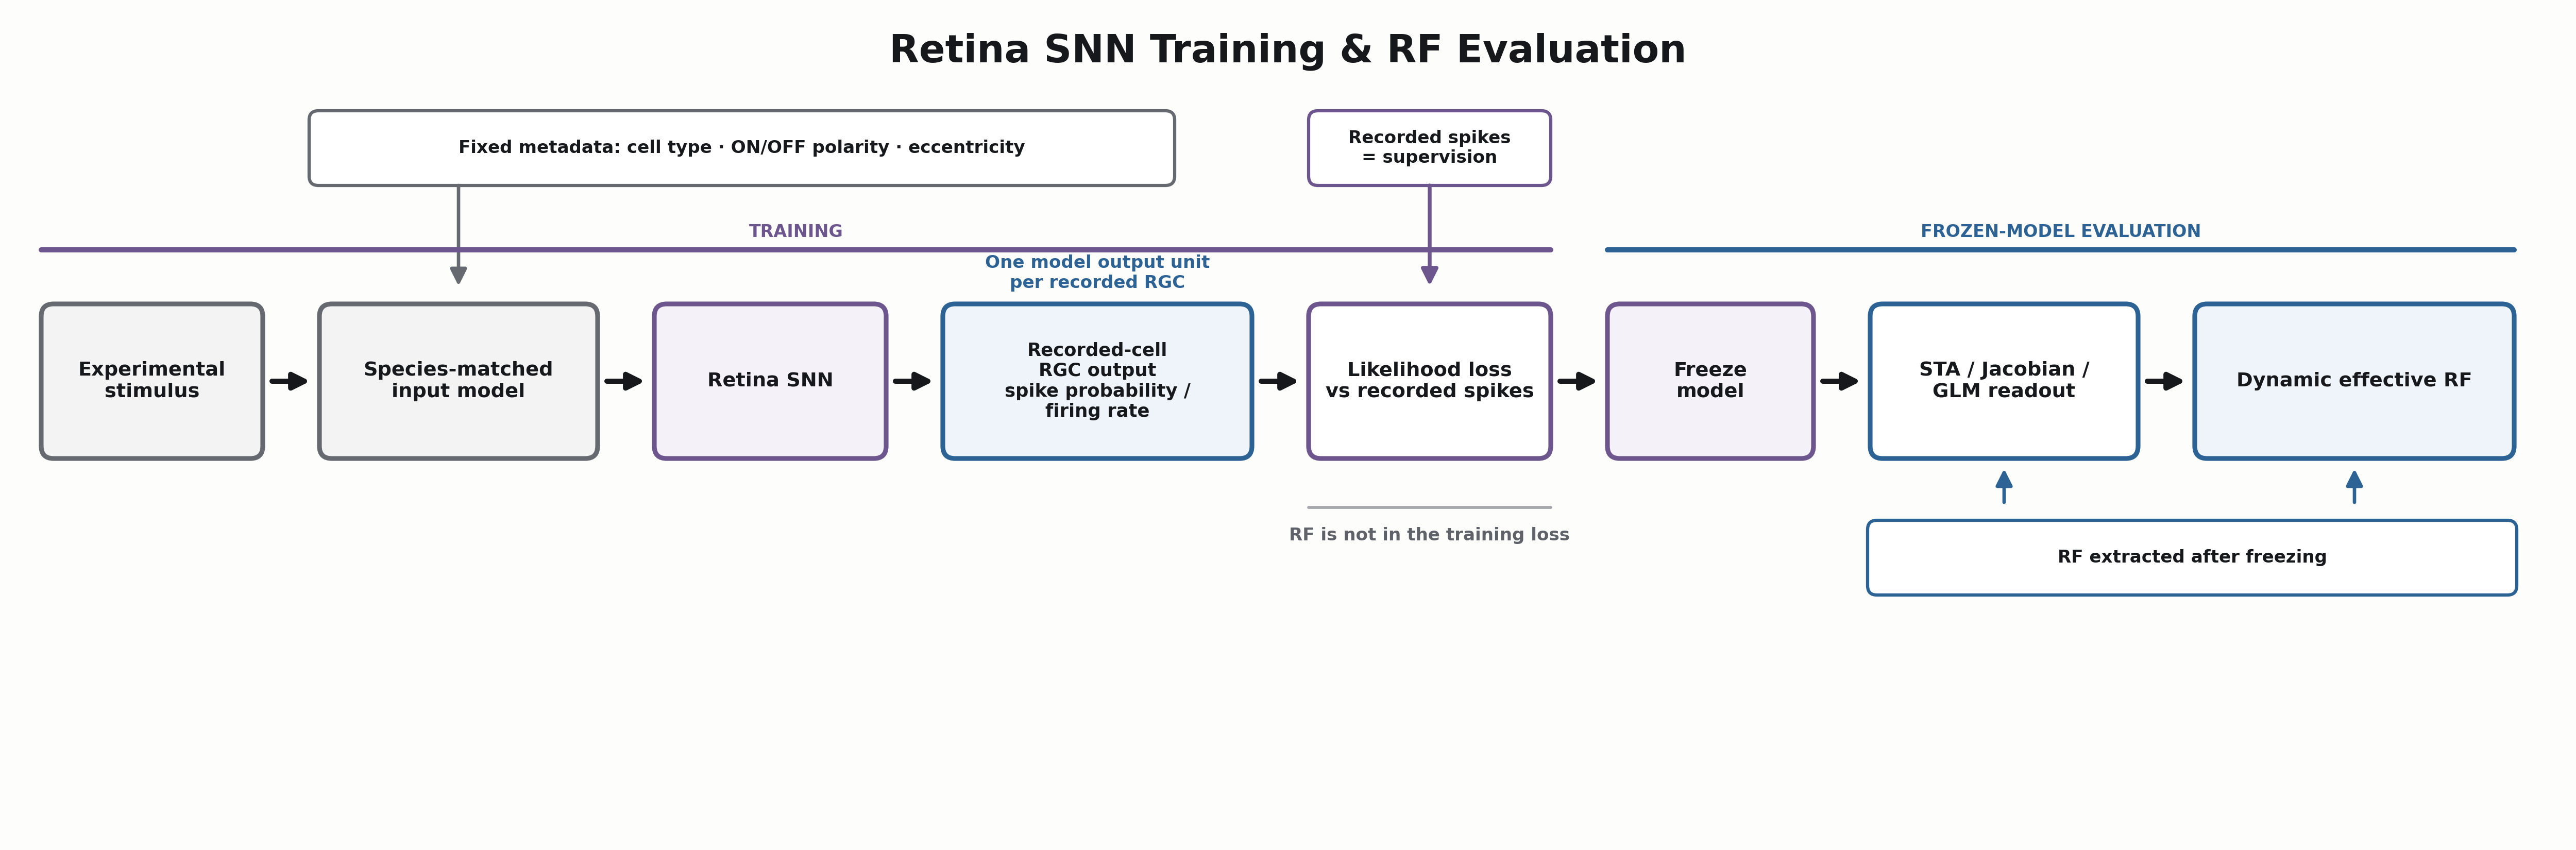
\includegraphics[width=\textwidth]
  {assets/retina_snn_training_evaluation_flow.png}
  \caption{Retina SNN の学習・評価フロー。各記録 RGC に
  一つの model output unit を対応させ、cell type、ON/OFF polarity、
  eccentricity は
  固定 metadata とする。recorded spike を教師信号として likelihood loss
  を計算し、RF は loss に含めず、モデル凍結後に
  STA、Jacobian、GLM readout から抽出する。}
  \label{fig:training-evaluation-flow}
\end{figure*}

\section{信号フローの解釈}

\subsection{入力と錐体}

自然画像は ISETBio により網膜面の光学像へ変換され、
L、M、S 錐体の励起として表現される。図中の三つの錐体は
三種類の入力チャネルを表す簡略記号である。
ヒトとマカクでは錐体密度や L:M 比が同一ではないため
\cite{curcio1990,hofer2005,packer1989,munds2022}、
モデルでは物種別パラメータを明示的に切り替える必要がある。

\subsection{水平細胞と双極細胞}

マカク H1 水平細胞は主に L/M 錐体入力を受け、S 錐体入力は
弱い、または測定上認められない。一方、H2 は S 錐体入力が強い
\cite{dacey1996}。本研究の主経路は輝度処理を担う L/M--H1 系であるため、
図では H1 を主ノードとして示し、S$\rightarrow$H1 は破線で示した。

錐体終末から ON 双極細胞への伝達は mGluR6 を介する符号反転、
OFF 双極細胞への伝達は AMPA/kainate 型受容体を介する符号保存として
表現する。双極細胞の center--surround は H1 を含む外網状層回路に
依存する。H1 は狭い直接入力成分と広い coupled network 成分で表現する。

\newpage
\subsection{アマクリン細胞と RGC}

アマクリン細胞は多数のサブタイプを含む
\cite{masland2012}。現在のモデルではサブタイプが一意に確定していないため、
図では ``Local amacrine cell'' とした。双極細胞から RGC への直接経路を
主経路として残し、アマクリン細胞はそれを遮断しない並列抑制経路として示す。
したがって、アマクリン細胞に単一の普遍的な受容野径や遅延を与えることはしない。

RGC は ON-center と OFF-center に分け、軸索出力を視神経の
スパイク列として示す。midget と parasol の数値は偏心度、
測定条件、解剖学的樹状野と生理学的受容野の違いに依存するため、
表\ref{tab:physiology}で条件とともに整理する。

\clearpage
\onecolumn

\begin{landscape}
\section{細胞間の接続関係}

\captionof{table}{錐体から RGC までの分布、収束、発散、接続関係。
一つの定数で表現できない項目は \unknownmark{} とした。}
\label{tab:connectivity}

\scriptsize
\setlength{\tabcolsep}{3.5pt}
\begin{tabularx}{0.98\linewidth}{
  >{\raggedright\arraybackslash}p{0.115\linewidth}
  >{\raggedright\arraybackslash}p{0.175\linewidth}
  >{\raggedright\arraybackslash}p{0.235\linewidth}
  >{\raggedright\arraybackslash}p{0.245\linewidth}
  >{\raggedright\arraybackslash}p{0.13\linewidth}}
\toprule
\textbf{部位・物種} &
\textbf{経路} &
\textbf{分布・収束} &
\textbf{発散・下流接続} &
\textbf{証拠種別・文献} \\
\midrule

発達期ヒト中心窩 &
L/M cone $\rightarrow$ ON midget bipolar
$\rightarrow$ ON midget RGC &
serial EM connectome が受容野中心の single-cone resolution を示す。
各 ON private-line branch では cone : bipolar : RGC $=1:1:1$。 &
一つの cone は ON 系と OFF 系へ分岐する。
周辺機構には水平細胞回路が加わる。 &
解剖学・接続構造
\cite{zhang2020} \\

発達期ヒト中心窩 &
L/M cone $\rightarrow$ OFF midget bipolar
$\rightarrow$ OFF midget RGC &
OFF private-line branch も受容野中心で
cone : bipolar : RGC $=1:1:1$ の single-cone resolution を形成する。 &
ON 系と並列に構成され、同一 cone から極性別経路が生じる。 &
解剖学・接続構造
\cite{zhang2020} \\

中心窩・マカク &
L/M cone $\rightarrow$ midget bipolar
$\rightarrow$ midget RGC &
受容野中心は single-cone input を保つ。
L/M 経路で bipolar--RGC 間の興奮性シナプス数に差が報告される。 &
cone は ON/OFF midget bipolar へ分岐し、
各 branch が対応する midget RGC 中心を駆動する。 &
解剖学的データ
\cite{calkins1994} \\

中心網膜から周辺網膜・マカク &
cone / midget bipolar $\rightarrow$ midget RGC &
中心部は single-cone center。偏心度の増加に伴い、
複数の cone--midget bipolar 入力が一つの midget RGC 中心へ収束する。 &
収束数と spatial support は偏心度に依存する。
全網膜共通の固定比率は \unknownmark{}。 &
解剖学的データ + 生理測定
\cite{wool2018} \\

全網膜・マカク &
cone $\leftrightarrow$ H1/H2 horizontal cell &
水平細胞 soma は regular mosaic を形成する。
一つの cone は各型 3--5 個の水平細胞と接触するという解剖学的推定。 &
H1 は L/M 優位、H2 は S 強入力と L/M 弱入力を持つ。
network coupling と cone-terminal feedback が広い空間統合を作る。 &
解剖学的データ + マカクでの直接測定
\cite{wassle1989,dacey1996} \\

中周辺部・マカク &
cone $\rightarrow$ DB3 diffuse bipolar
$\rightarrow$ OFF parasol RGC &
一つの OFF parasol RGC に約 50 個の DB3、約 500 シナプス。
DB3 集団の上流は約 250 cone と推定される。 &
diffuse bipolar pooling が midget 系より広い
parasol center support を構成する。 &
解剖学的データ
\cite{jacoby2000} \\

未確定サブタイプ &
ON/OFF bipolar $\rightarrow$ local amacrine
$\dashv$ bipolar/RGC &
アマクリン細胞は多数のサブタイプを含み、空間範囲、
収束数、時間特性がサブタイプごとに異なる。 &
抑制性の並列経路を形成する。generic node に対応する
サブタイプ、収束比、発散比は \unknownmark{}。 &
不明（サブタイプ依存）
\cite{masland2012,protti2014} \\

\bottomrule
\end{tabularx}

\vspace{0.7\baselineskip}
\noindent\textbf{表の説明：}
中心窩の $1:1:1$ は、発達期ヒト中心窩の serial EM で示された
\textbf{各 ON/OFF private-line branch の受容野中心}を指す。
cone から ON/OFF への分岐、水平細胞を介する周辺機構、偏心度に伴う
midget 経路の収束を同時に扱う。発達段階、物種、偏心度、細胞サブタイプを
接続比のキーとする。\unknownmark{} は、generic amacrine node に
一つの細胞数比を割り当てるためのサブタイプ情報が不足していることを示す。

\end{landscape}

\clearpage
\section{パラメータ決定方針}

パラメータは由来と選定方法に基づいて五区分に分ける。

\begin{center}
\centering
\captionof{table}{パラメータ区分。}
\label{tab:parameter-class}
\small
\setlength{\tabcolsep}{5pt}
\begin{tabularx}{0.92\textwidth}{
  >{\raggedright\arraybackslash}p{0.20\textwidth}
  >{\raggedright\arraybackslash}p{0.31\textwidth}
  Y}
\toprule
\textbf{区分} & \textbf{決定原理} & \textbf{代表例} \\
\midrule
DATA-FIXED &
データファイルと実験プロトコルから決定し、学習中は固定 &
時間軸、cone/cell position、cell mapping、stimulus split \\
BIO-FIXED &
高信頼の生理・解剖知見からトポロジー、極性、順序を固定 &
ON/OFF 分岐、局所接続、興奮/抑制符号、直接 bipolar$\rightarrow$RGC 経路 \\
BOUNDED-LEARNED &
文献値から初期値、上下限、型間順序を設定し、記録応答から推定 &
時定数、gain、threshold、adaptation、local spatial weight \\
VALIDATION-TUNED &
validation set と training diagnostics により選択 &
learning rate、BPTT 長、gradient clipping、regularization weight \\
POST-HOC &
モデル凍結後に測定し、loss へ入力しない &
RF center/surround、latency、dynamicity、type asymmetry \\
\bottomrule
\end{tabularx}
\end{center}

\clearpage

\begin{landscape}
\section{既知・未知の生理データ}

\captionof{table}{Retina SNN に関係する生理・解剖データの整理。
直接比較できる値が選定できていない欄は \unknownmark{} とした。}
\label{tab:physiology}

\scriptsize
\setlength{\tabcolsep}{2.8pt}
\begin{tabularx}{0.98\linewidth}{
  >{\raggedright\arraybackslash}p{0.095\linewidth}
  >{\raggedright\arraybackslash}p{0.175\linewidth}
  >{\raggedright\arraybackslash}p{0.215\linewidth}
  >{\raggedright\arraybackslash}p{0.215\linewidth}
  >{\raggedright\arraybackslash}p{0.14\linewidth}
  >{\raggedright\arraybackslash}p{0.075\linewidth}}
\toprule
\textbf{細胞・指標} &
\textbf{ヒト} &
\textbf{マカク} &
\textbf{測定条件・定義上の注意} &
\textbf{証拠 / モデル用途} &
\textbf{文献} \\
\midrule

錐体密度 &
ピーク平均 199,000 cones/mm$^2$（100,000--324,000）、
総数平均 4.6 million（4.08--5.29 million）。 &
\species{M. nemestrina}：ピーク平均 210,000 cones/mm$^2$
（190,000--260,000）、総数平均 3.1 million（2.8--3.3 million）。 &
いずれも postmortem whole-mount anatomy。ピーク位置と個体差を伴う。 &
解剖学的データ / DATA-FIXED。物種・偏心度別の geometry prior。 &
\cite{curcio1990,packer1989} \\

L:M 比・S 錐体割合 &
L:M $=1.1:1$--$16.5:1$。
約 $1^{\circ}$ で S cone $5.72\pm0.69\%$。 &
\species{M. mulatta}：L:M $=1.03:1\pm0.02$。
S-related expression ratio $0.143:1\pm0.002$。 &
ヒトは adaptive-optics imaging + densitometry。
マカク値は foveal opsin mRNA ddPCR による expression proxy。 &
ヒトでの直接測定 + 間接測定 / species-specific prior。 &
\cite{hofer2005,munds2022} \\

錐体応答時間 &
Dim-flash \Tpeak{} $\approx20$ ms。 &
5,000 R*/cone/s：L 36.7、M 36.3、S 45.3 ms。
50,000 R*/cone/s：L 33.1、M 34.1、S 44.5 ms。 &
ヒトは in vivo paired-flash ERG とモデルによる photocurrent 推定。
マカクは単一錐体電位応答。\Tpeak{} と synaptic delay は別指標。 &
間接測定 + マカクでの直接測定 / temporal bound と POST-HOC 比較。 &
\cite{vanhateren2006,baudin2019} \\

H1 入力選択性 &
直接生理の選択値：\unknownmark{}。 &
H1 は L/M 入力、測定上 S 入力なし又は極めて弱い。
H2 は S 強入力 + L/M 弱入力。 &
マカクの生理・解剖結果。ヒト profile では cross-species prior として記録する。 &
マカクでの直接測定 / BIO-FIXED（入力選択性と符号）。 &
\cite{dacey1996} \\

H1 受容野と時間 &
生理的 RF：\unknownmark{}。
時間：\unknownmark{}。 &
combined RF diameter 122 $\mu$m（偏心度 4 mm）、
309 $\mu$m（11 mm）。H1 は cone より \dTpeak{} $\approx4$ ms 遅い。 &
in vitro macaque retina。RF は狭い直接成分 + 広い coupled 成分。
4 ms は同一研究条件内の相対 peak latency。 &
マカクでの直接測定 / spatial bound、temporal POST-HOC。 &
\cite{packer2002,smith2001} \\

Midget bipolar RF &
直接生理 RF：\unknownmark{}。
時間：\unknownmark{}。 &
center diameter 42 $\mu$m（31--51）、
surround diameter 467 $\mu$m（432--515）。
時間：\unknownmark{}。 &
peripheral in vitro macaque retina。
diameter $=2\times$ Gaussian radius。 &
不明 + マカクでの直接測定 / BOUNDED-LEARNED spatial support。 &
\cite{dacey2000} \\

Diffuse bipolar RF &
直接生理 RF：\unknownmark{}。
時間：\unknownmark{}。 &
center diameter 92 $\mu$m（74--114）、
surround diameter 743 $\mu$m（594--1048）。
時間：\unknownmark{}。 &
peripheral in vitro macaque retina。
diameter $=2\times$ Gaussian radius。 &
不明 + マカクでの直接測定 / BOUNDED-LEARNED spatial support。 &
\cite{dacey2000} \\

Cone$\rightarrow$bipolar の時間 &
直接 synaptic delay：\unknownmark{}。 &
直接 synaptic delay：\unknownmark{}。 &
ON/OFF の受容体機構は既知でも、図の各層へ一律に与えられる
比較可能な delay 値は選定していない。 &
不明 / polarity BIO-FIXED、時間特性 BOUNDED-LEARNED。 &
--- \\

Generic local amacrine &
RF：\unknownmark{}、delay：\unknownmark{}。 &
RF：\unknownmark{}、delay：\unknownmark{}。 &
サブタイプ、刺激、順応状態、記録法に依存する。
generic node にはサブタイプ共通値を設定しない。 &
不明 / inhibitory sign BIO-FIXED、動態 BOUNDED-LEARNED。 &
\cite{masland2012,protti2014} \\

Midget / parasol RGC &
解剖学的 dendritic-field diameter：
$D_{\mathrm{midget}}=8.64E^{1.04}$、
$D_{\mathrm{parasol}}=70.2E^{0.65}$。
生理 RF・応答時間：\unknownmark{}。 &
P/M の center と surround は偏心度とともに増大し、
M center radius は近傍 P の約 2 倍。 &
ヒト式は $D$：$\mu$m、$E$：mm で、temporal/superior/inferior retina の
形態データ。マカク値は生理測定。 &
解剖学的データ + マカクでの直接測定 / spatial prior と POST-HOC RF。 &
\cite{dacey1992,croner1995} \\

Midget RGC 時間 &
\unknownmark{}。 &
STA \Tpeak{}：foveal $67\pm6$ ms、
central $53\pm6$ ms、peripheral $37\pm4$ ms。 &
ex vivo macaque retina。刺激・STA 定義に依存し、
錐体 \Tpeak{} や synaptic delay と直接加算しない。 &
マカクでの直接測定 / POST-HOC temporal RF。 &
\cite{sinha2017} \\

ON/OFF parasol 非対称性 &
\unknownmark{}。 &
ON RF diameter は OFF より約 20\% 大きい。
ON の peak/trough/zero-crossing 時間は OFF より 10--20\% 短い。 &
in vitro white-noise response。相対差として用いる。 &
マカクでの直接測定（機能的分類）/ POST-HOC asymmetry。 &
\cite{chichilnisky2002} \\

\bottomrule
\end{tabularx}

\vspace{0.7\baselineskip}
\noindent\textbf{表の説明：}
\unknownmark{} は、選定した一次文献の範囲で、
同じ細胞サブタイプ、偏心度、刺激、順応状態、測定定義を満たす
直接比較可能な値を確定していないことを示す。
物種間の値は source species を保持した proxy として管理する。
\Tpeak{}、\dTpeak{}、時定数 $\tau$、直接 synaptic delay は
別々のフィールドに保存する。ヒト RGC の式は解剖学的樹状野として管理する。
証拠種別は、測定対象と測定方法が直接分かる日本語で記載する。

\end{landscape}

\clearpage
\onecolumn

\section{物種別の生理証拠フロー}

緑の○は、選定した一次文献に対象物種の直接的な解剖学的または
生理学的証拠が存在する箇所を示す。赤の×は、同じ細胞型、偏心度、
刺激条件、測定定義で直接比較できる対象物種の証拠を確定していない
箇所を示す。赤の×は回路自体の不存在を意味しない。

\begin{center}
  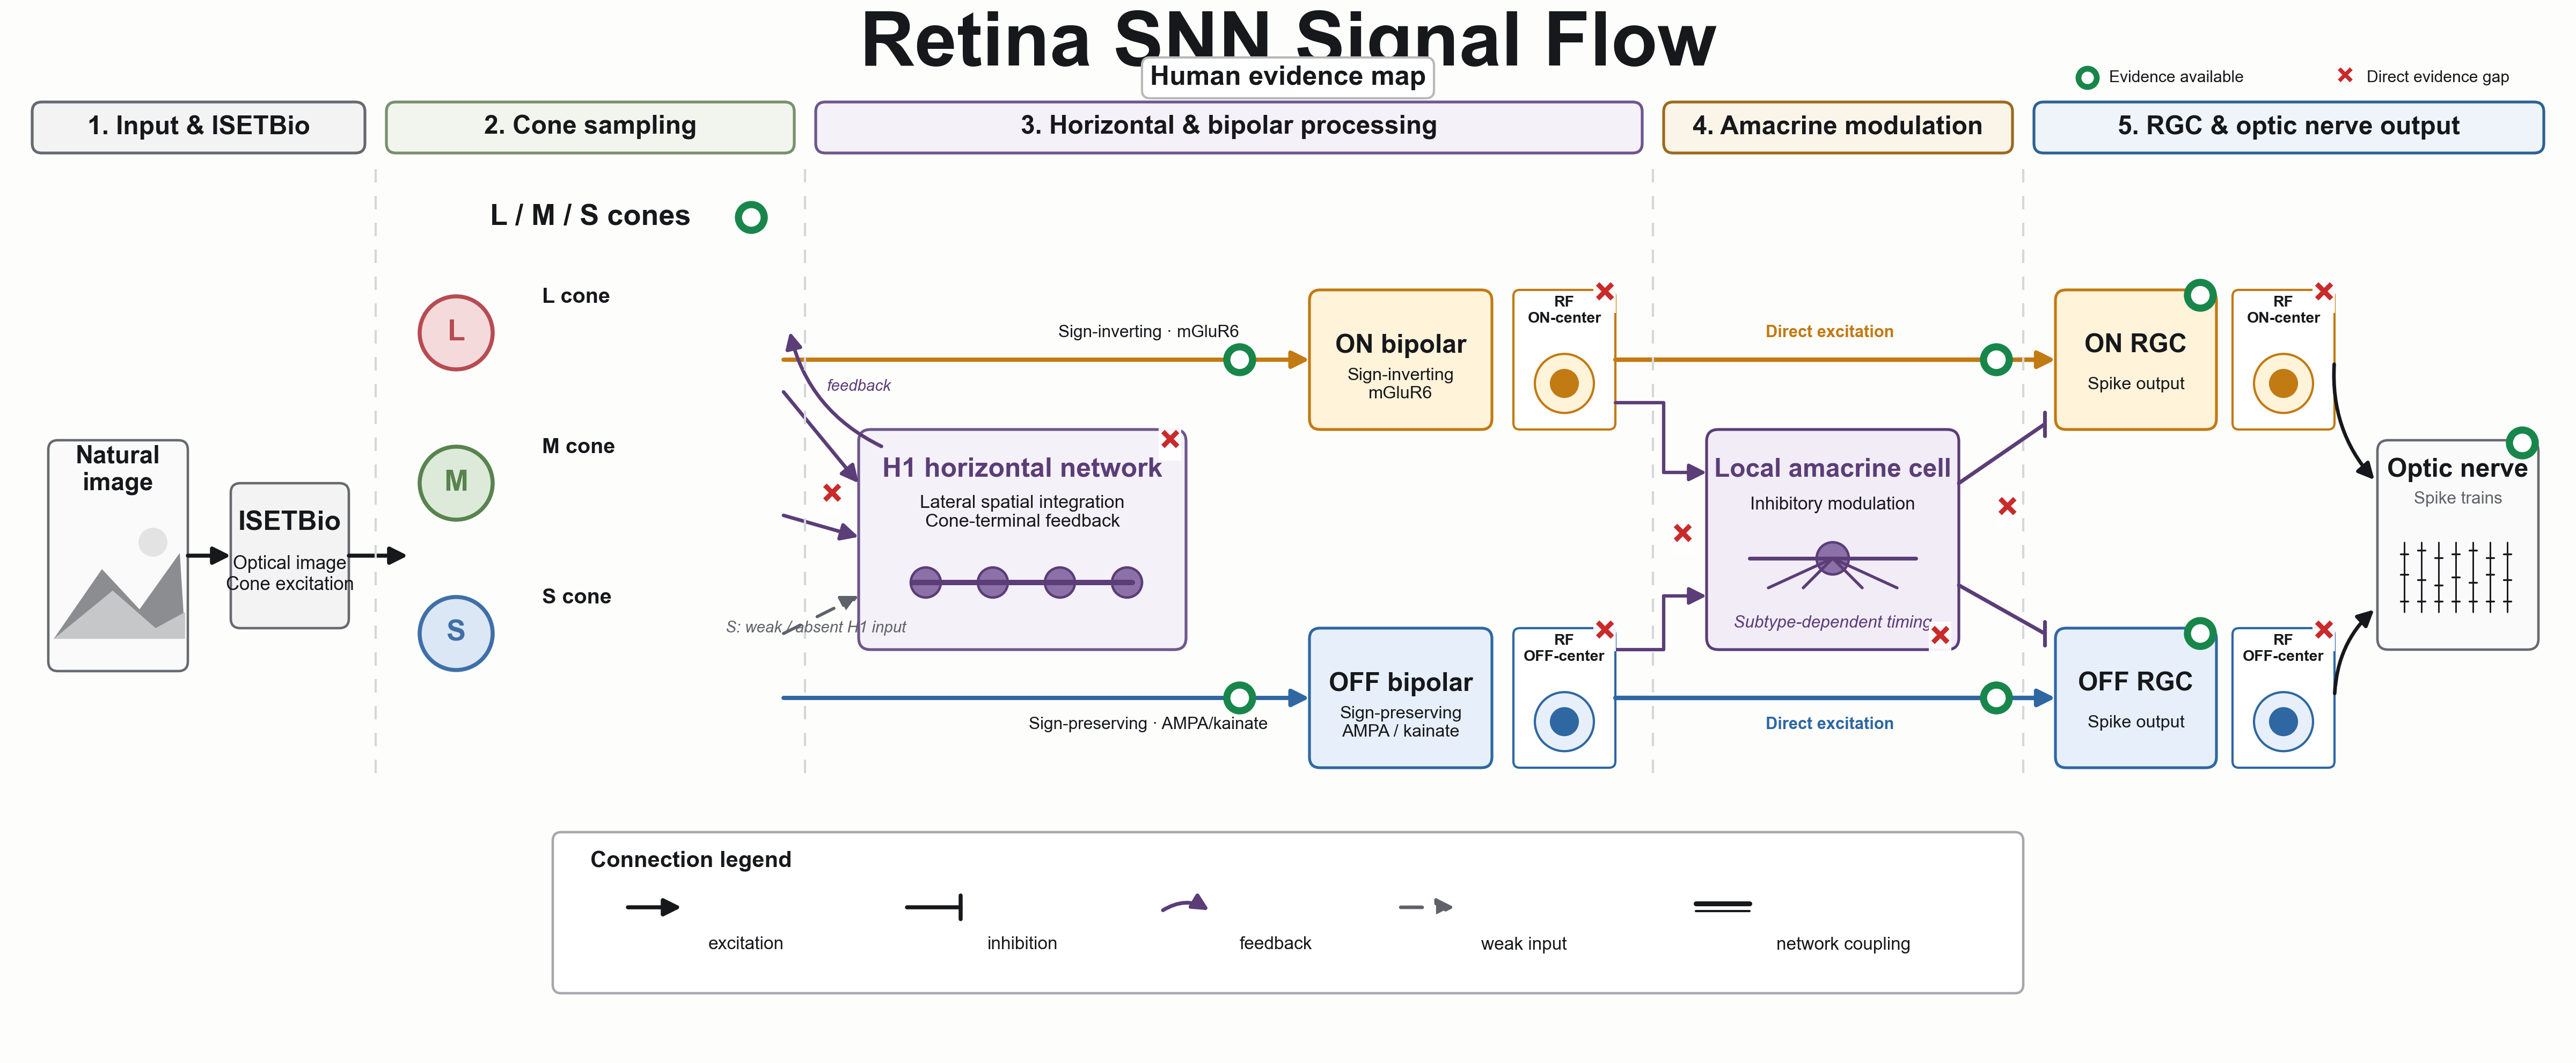
\includegraphics[width=\textwidth]{assets/retina_snn_evidence_flow_human.png}
  \captionof{figure}{ヒトにおける生理証拠の分布。
  緑の○は証拠あり、赤の×は直接比較可能な証拠が未確定であることを示す。}
  \label{fig:evidence-flow-human}
\end{center}

\vspace{0.8\baselineskip}

\begin{center}
  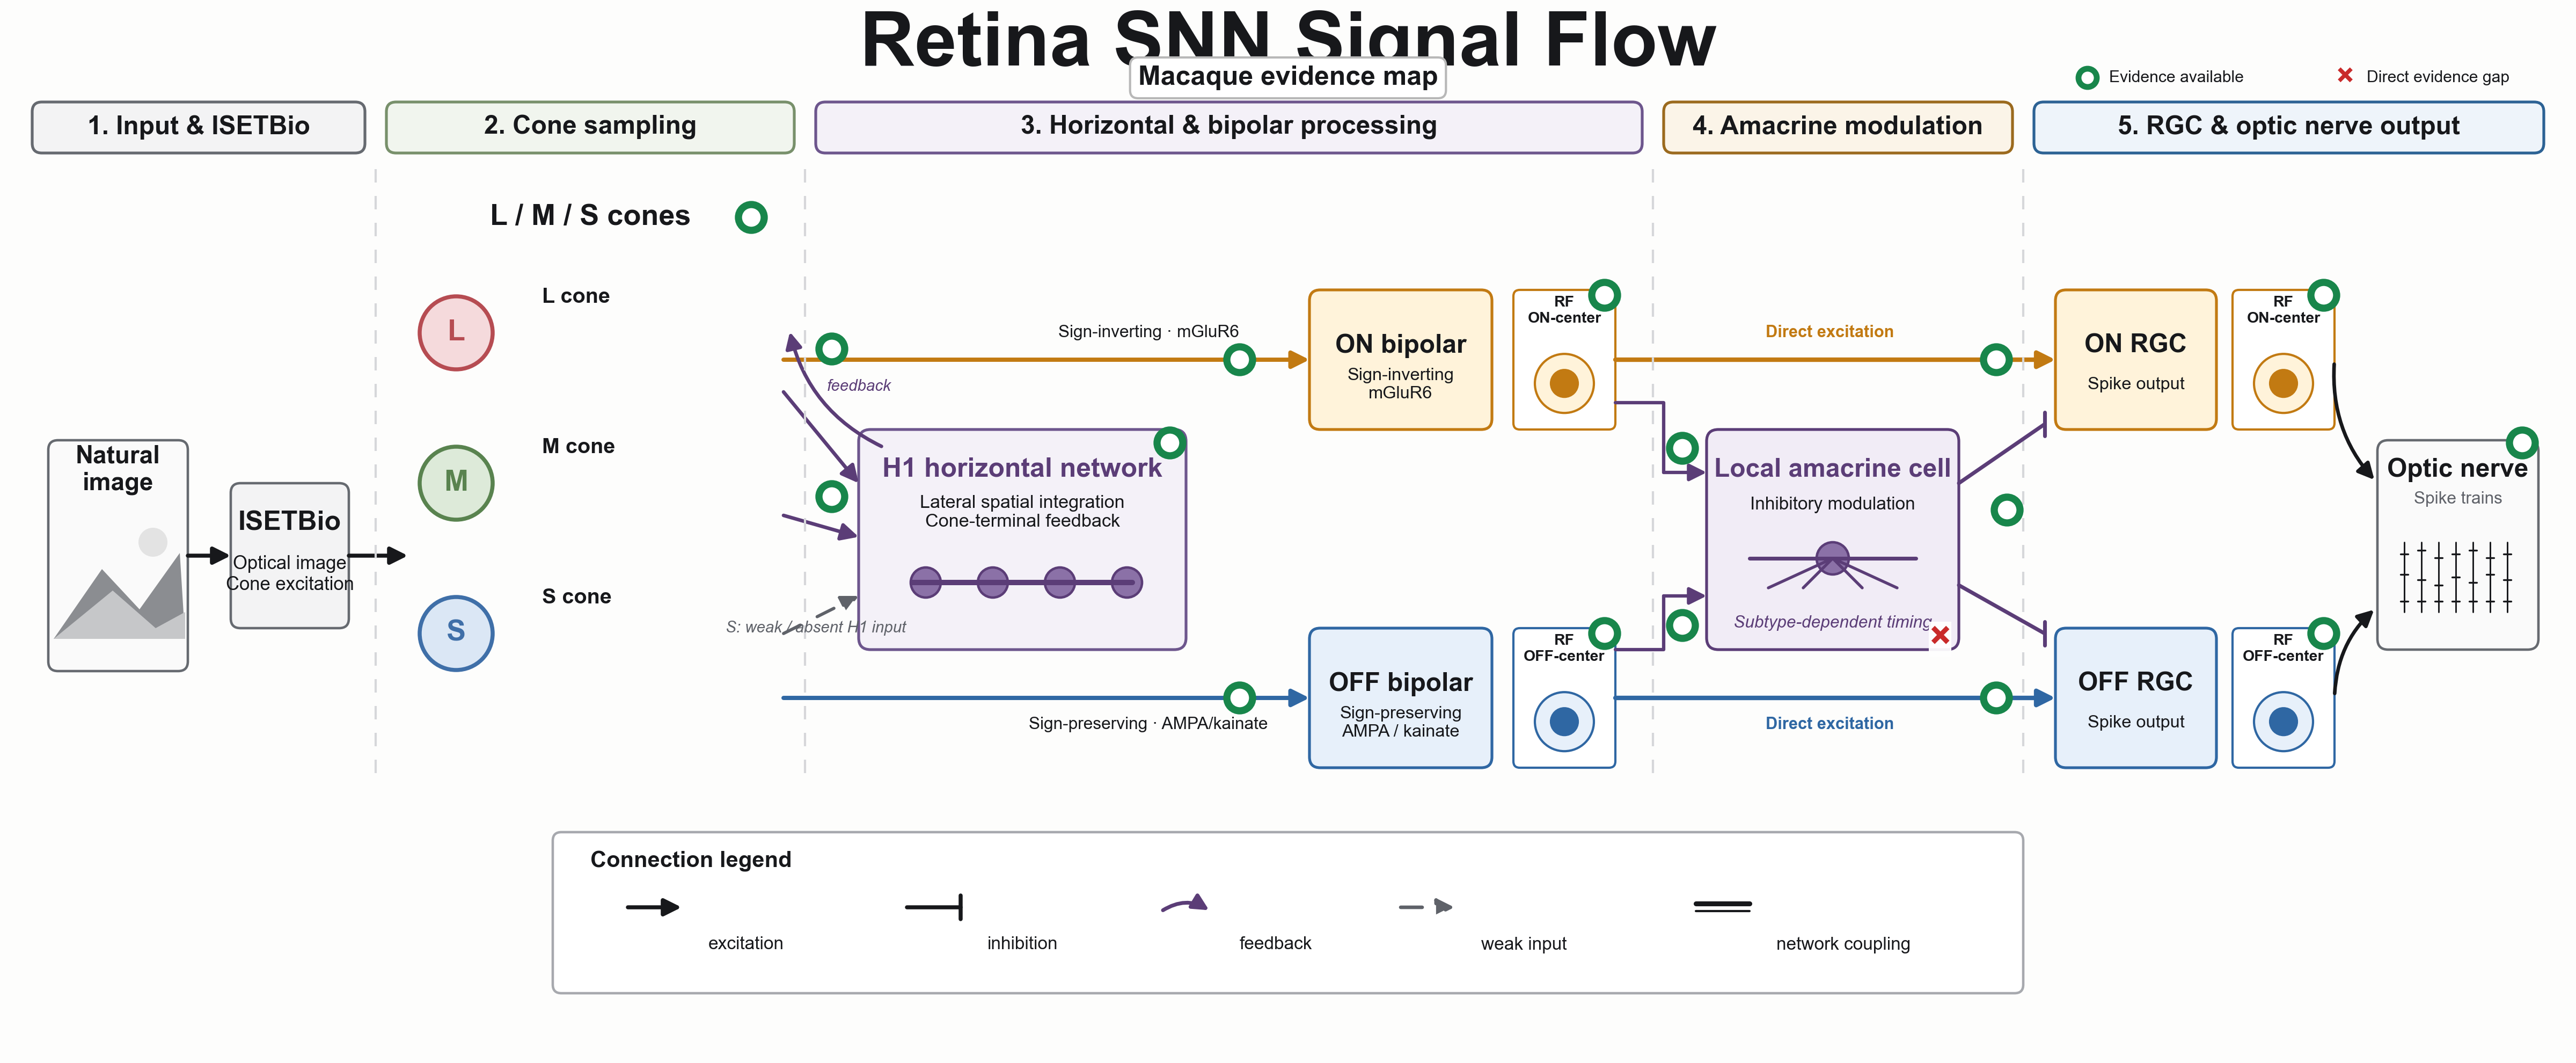
\includegraphics[width=\textwidth]{assets/retina_snn_evidence_flow_macaque.png}
  \captionof{figure}{マカクにおける生理証拠の分布。
  緑の○は証拠あり、赤の×は直接比較可能な証拠が未確定であることを示す。}
  \label{fig:evidence-flow-macaque}
\end{center}

\clearpage

\section{対象物種と学習データ}

\subsection{物種プロファイル}

方法評価の主設定にはマカクを用いる。マカクでは RGC の記録応答、
受容野、時間特性、内網膜回路に関する直接生理データが比較的豊富であり、
記録 spike とモデル unit を対応させた system identification が可能である。
ヒト設定は ISETBio optics、ヒト cone geometry、ヒト解剖データを持つ
独立プロファイルとして構築する。内網膜の type-level dynamics は
マカクで学習した値を感度分析条件ごとの固定値として転移し、
ヒト固有の学習済みパラメータとはみなさない。

\begin{center}
\centering
\captionof{table}{物種と実験条件の運用方針。}
\label{tab:species-policy}
\small
\setlength{\tabcolsep}{4pt}
\begin{tabularx}{0.98\textwidth}{
  >{\raggedright\arraybackslash}p{0.14\textwidth}
  >{\raggedright\arraybackslash}p{0.20\textwidth}
  >{\raggedright\arraybackslash}p{0.20\textwidth}
  >{\raggedright\arraybackslash}p{0.23\textwidth}
  Y}
\toprule
\textbf{設定} &
\textbf{入力と生理データ} &
\textbf{学習・評価} &
\textbf{研究上の役割} &
\textbf{主要リスク} \\
\midrule
Macaque-primary &
macaque-specific stimulus geometry、cone response、RGC spike、
cell type、polarity、eccentricity &
recorded spike likelihood、dynamic RF、mechanism ablation &
提案手法の主評価、parameter identification、baseline 比較 &
種・偏心度・in vivo/ex vivo 条件の混在 \\

Human-transfer &
human optics、human cone mosaic、human anatomy &
type-level parameter の固定転移、感度分析、RF range と挙動の確認 &
ヒト視覚への適用可能性、species transfer の評価 &
inner-retinal direct physiology と spike data の不足 \\

Cross-species pilot &
human ISETBio input と macaque physiology proxy &
pipeline check、scale sensitivity、parameter-recovery control &
実装検証と仮説形成 &
一つの生物個体・物種を表す結果として解釈できる範囲が狭い \\
\bottomrule
\end{tabularx}
\end{center}

in vivo データでは対象物種の optics を含む visual-space 座標を用いる。
ex vivo retina データでは網膜面刺激と retinal-space 座標を用いる。
二つの測定条件は独立した observation model として保存する
\cite{cottaris2026}。

\subsection{学習対象}

主学習対象はマカクの記録 RGC spike response である。データ契約は
\texttt{cone\_response [stimulus,time,cone]}、
\texttt{spike\_counts [stimulus,trial,time,cell]}、
\texttt{valid\_mask}、\texttt{time\_axis\_seconds}、
cone/cell position、cell type、ON/OFF polarity、eccentricity を保持する。
target kind に応じて Bernoulli または Poisson negative log-likelihood を用い、
cell ごとの有効サンプル数をそろえて平均する。

synthetic teacher は parameter recovery、符号回復、実装の健全性を確認する。
記録データによる held-out likelihood と RF 評価を生理的主張の判定に用いる。
future cone prediction は normative control、cone reconstruction は
information-preservation control として位置づける。RF 形状は training target
に含めず、凍結後のモデル応答から STA、Jacobian、GLM readout で推定する。

\clearpage
\onecolumn

\subsection*{ヒト プロファイル のパラメータ決定方針}

\captionof{table}{ヒト プロファイル における固定項目、学習項目、決定方法。}
\label{tab:model-policy-human}

\scriptsize
\renewcommand{\arraystretch}{1.08}
\setlength{\tabcolsep}{2.5pt}
\begin{tabularx}{0.98\linewidth}{
  >{\raggedright\arraybackslash}p{0.14\linewidth}
  >{\raggedright\arraybackslash}p{0.24\linewidth}
  >{\raggedright\arraybackslash}p{0.19\linewidth}
  Y}
\toprule
\textbf{対象} &
\textbf{具体的内容} &
\textbf{区分} &
\textbf{固定・学習方法} \\
\midrule

入力・形態\newline（固定） &
human optics、cone mosaic、eccentricity、
midget/parasol dendritic field &
DATA-FIXED + BIO-FIXED &
ISETBio のヒト入力とヒト解剖データを固定する。
マカクの密度・RF 数値で置き換えない \\

H1 horizontal\newline（転移値を固定・感度分析） &
L/M input、feedback sign、direct/coupled radius、gain、$\tau_H$ &
BIO-FIXED + DATA-FIXED（転移値） &
回路上の入力選択性、feedback 符号、局所 coupling を固定する。
ヒトの直接 RF・時間値は不明なため、マカクで決定した radius、gain、
$\tau_H$ を条件ごとに固定し、範囲内で感度分析する \\

Bipolar cells\newline（転移値を固定・感度分析） &
ON/OFF polarity、midget/diffuse support、center/surround、
gain、$\tau_B$、rectification &
BIO-FIXED + DATA-FIXED（転移値） &
ON/OFF の符号と foveal midget の解剖学的構造を固定する。
ヒトの直接 RF・時間値は不明なため、マカクで決定した spatial support と
動態値を条件ごとに固定し、範囲内で感度分析する \\

Amacrine dynamics\newline（転移値を固定・感度分析） &
inhibitory sign、parallel pathway、subtype、
local radius、gain、$\tau_A$ &
BIO-FIXED + DATA-FIXED（転移値） &
抑制符号と並列経路のみ固定する。ヒトの subtype 別直接値が不明なため、
マカクで決定した radius、gain、$\tau_A$ を条件ごとに固定する。
subtype をヒト固有の確定値として解釈しない \\

RGC type prior\newline（固定） &
ON/OFF、midget/parasol、dendritic field、eccentricity &
DATA-FIXED + BIO-FIXED &
ヒト解剖に基づく type、polarity、空間配置を固定する。
記録細胞 metadata がない場合は cell identity を仮定しない \\

RGC dynamics\newline（マカクから転移して固定） &
局所入力支持範囲、sustained mix、membrane/adaptation $\tau$、
adaptation gain、threshold、subunit time/gain &
DATA-FIXED（転移値） &
マカクで学習した type-level parameter を固定して転移する。
cell-specific residual は学習しない。ヒト RGC 応答を導入する場合は、
別の human-fitting experiment として再定義する \\

出力 likelihood\newline（現段階では使用しない） &
human RGC spike/rate、cell bias、observed-spike history &
該当なし &
現在の human-transfer プロファイル には直接対応するヒト RGC 記録がないため、
spike likelihood fitting と cell-specific parameter 学習を行わない \\

転移・感度分析\newline（感度分析で設定） &
transfer parameter set、species scaling、parameter range &
VALIDATION-TUNED &
マカク転移値を中心に複数の固定条件を比較する。
予測性能だけで一つの条件をヒト真値として選ばない \\

RF 指標\newline（転移後に評価） &
center、surround、latency、polarity、dynamicity &
POST-HOC &
human-transfer model 凍結後に抽出し、ヒト解剖値とは比較するが、
直接ヒト生理 RF としては解釈しない \\
\bottomrule
\end{tabularx}

\vspace{0.6\baselineskip}
\noindent\textbf{表の説明：}
ヒト プロファイル は human optics、cone geometry、解剖データを保持する。
現段階では、内網膜 dynamics と cell-specific parameter を
ヒトデータから学習しない。マカク由来値は source species を保持した固定転移値とし、
複数条件の感度分析に用いる。したがって、本表の転移値を
ヒト固有の生理パラメータまたは学習結果として解釈しない。

\clearpage
\subsection*{マカク プロファイル のパラメータ決定方針}

\captionof{table}{マカク プロファイル における固定項目、学習項目、決定方法。}
\label{tab:model-policy-macaque}

\scriptsize
\renewcommand{\arraystretch}{1.08}
\setlength{\tabcolsep}{2.5pt}
\begin{tabularx}{0.98\linewidth}{
  >{\raggedright\arraybackslash}p{0.14\linewidth}
  >{\raggedright\arraybackslash}p{0.24\linewidth}
  >{\raggedright\arraybackslash}p{0.19\linewidth}
  Y}
\toprule
\textbf{対象} &
\textbf{具体的内容} &
\textbf{区分} &
\textbf{固定・学習方法} \\
\midrule

入力・記録条件\newline（固定） &
macaque stimulus geometry、cone response、cell identity、
eccentricity、in vivo/ex vivo &
DATA-FIXED &
各記録データの物種、偏心度、刺激座標、時間軸、cell mapping を固定する。
in vivo と ex vivo を同じ observation model に混合しない \\

H1 horizontal\newline（一部固定・モデル学習） &
L/M input、feedback sign、direct/coupled radius、
coupling strength、gain、$\tau_H$ &
BIO-FIXED + BOUNDED-LEARNED &
L/M 優位入力、feedback 符号、局所 coupling topology を固定する。
表\ref{tab:physiology}のマカク RF・相対時間を範囲として、
radius は離散選択、gain と $\tau_H$ は記録応答から学習する \\

Bipolar cells\newline（一部固定・モデル学習） &
ON/OFF polarity、midget/diffuse support、center/surround、
gain、$\tau_B$、rectification &
BIO-FIXED + BOUNDED-LEARNED &
ON/OFF の符号、受容体機構、局所 topology を固定する。
マカク RF 範囲内で spatial support を離散選択し、
gain、$\tau_B$、rectification を記録応答から学習する \\

Amacrine dynamics\newline（一部固定・モデル学習） &
inhibitory gain、time scale、local radius、feedback target &
BIO-FIXED + BOUNDED-LEARNED &
抑制符号と並列経路を固定する。generic amacrine の subtype は仮定せず、
radius は離散選択、gain と $\tau_A$ はマカク RGC 応答から有界学習する \\

RGC type prior\newline（固定） &
ON/OFF、midget/parasol、cell identity、eccentricity &
DATA-FIXED + BIO-FIXED &
記録 metadata の type label、polarity、cell identity、eccentricity を固定し、
同じ type の base parameter を共有する \\

RGC learnable state\newline（モデル学習） &
局所入力支持範囲、sustained mix、membrane/adaptation $\tau$、
adaptation gain、threshold、subunit time/gain &
BOUNDED-LEARNED &
マカク生理範囲内で type-level parameter を学習し、
cell-specific residual を小さく正則化する \\

出力 likelihood\newline（一部固定・モデル学習） &
Bernoulli/Poisson target、cell bias、observed-spike history &
DATA-FIXED + BOUNDED-LEARNED &
target kind は記録データ属性で固定する。
bias、history、readout weight はマカク RGC 応答から学習する \\

学習制御\newline（検証データで設定） &
learning rate、BPTT、gradient clipping、prior weights &
VALIDATION-TUNED &
マカク validation likelihood、gradient statistics、
state stability により選択する \\

RF 指標\newline（学習しない） &
center、surround、latency、polarity、dynamicity &
POST-HOC &
モデル凍結後に STA、Jacobian、GLM から抽出し、
偏心度と測定条件を合わせたマカク生理データと比較する \\
\bottomrule
\end{tabularx}

\vspace{0.6\baselineskip}
\noindent\textbf{表の説明：}
マカク　プロファイルは、本研究で内網膜 dynamics と RGC parameter を
記録応答から学習する主プロファイルであり、parameter identification と主評価に用いる。
学習可能量は type-level shared parameter と小さな cell-specific residual に分ける。
上下限は変換パラメータ化によって満たし、範囲端への集中を
parameter identifiability の警告として記録する。local support の半径は
連続重みと同時に自由化せず、マカク文献範囲内の離散 sweep で決定する。

\clearpage
\twocolumn

\section{比較実験と成功条件}

\subsection{比較モデル}

\begin{enumerate}
  \item LN / point-process GLM：標準的な解釈可能 RF baseline
  \item 同容量の無制約 NN/SNN：生理制約の寄与を測る baseline
  \item 全パラメータ固定の生理モデル：データ学習の寄与を測る baseline
  \item 生理制約付き部分学習モデル：提案手法
\end{enumerate}

GLM baseline は recorded spike に対する同一 split、同一 bin、
同一 likelihood で評価する \cite{pillow2008}。各 baseline は
readout capacity、unit 数、training budget を可能な範囲でそろえる。

\subsection{評価指標}

\begin{enumerate}
  \item held-out spike negative log-likelihood と calibration
  \item seed 間の RF center/surround、polarity、latency の安定性
  \item white noise と natural movie 間の RF 一致性
  \item contrast、luminance、stimulus statistics 変化への汎化
  \item 少数データ条件の sample efficiency
  \item learned parameter の bound occupancy と type-level reproducibility
  \item H1、bipolar、amacrine、RGC dynamics の経路特異的 ablation
\end{enumerate}

\subsection{成功条件}

提案手法は、無制約モデルに近い予測性能を保ち、RF の seed stability、
cross-stimulus generalization、生理範囲内のパラメータ、
経路特異的な消融効果を同時に示した場合に支持される。
高い spike likelihood と不安定な内部パラメータが併存する場合、
応答予測能力を報告し、機構同定の結論を保留する。


\section{まとめ}

本研究は、霊長類網膜の接続 topology、ON/OFF polarity、局所性、
細胞型、偏心度依存性を明示し、直接測定が不足する dynamics を
生理範囲内で学習する grey-box Retina SNN を扱う。
主実験は macaque recorded RGC spike fitting、ヒト設定は独立 transfer profile
として構成する。パラメータを DATA-FIXED、BIO-FIXED、
BOUNDED-LEARNED、VALIDATION-TUNED、POST-HOC に分け、
出力校正、RGC dynamics、上流 dynamics、joint fine-tuning の順に学習する。
dynamic effective RF は学習後に抽出し、GLM、無制約モデル、
全固定モデルとの比較、複数刺激、複数 seed、機構消融により評価する。

\begin{thebibliography}{99}
\small

\bibitem{maass1997}
W. Maass,
``Networks of spiking neurons: The third generation of neural network models,''
\textit{Neural Networks}, vol. 10, no. 9, pp. 1659--1671, 1997.
\url{https://doi.org/10.1016/S0893-6080(97)00011-7}

\bibitem{gerstner2014}
W. Gerstner, W. M. Kistler, R. Naud, and L. Paninski,
\textit{Neuronal Dynamics: From Single Neurons to Networks and Models of Cognition}.
Cambridge University Press, 2014.
\url{https://doi.org/10.1017/CBO9781107447615}

\bibitem{lecun2015}
Y. LeCun, Y. Bengio, and G. Hinton,
``Deep learning,''
\textit{Nature}, vol. 521, pp. 436--444, 2015.
\url{https://doi.org/10.1038/nature14539}

\bibitem{neftci2019}
E. O. Neftci, H. Mostafa, and F. Zenke,
``Surrogate gradient learning in spiking neural networks:
Bringing the power of gradient-based optimization to spiking neural networks,''
\textit{IEEE Signal Process. Mag.}, vol. 36, no. 6, pp. 51--63, 2019.
\url{https://doi.org/10.1109/MSP.2019.2931595}

\bibitem{eshraghian2023}
J. K. Eshraghian et al.,
``Training spiking neural networks using lessons from deep learning,''
\textit{Proc. IEEE}, vol. 111, no. 9, pp. 1016--1054, 2023.
\url{https://doi.org/10.1109/JPROC.2023.3308088}

\bibitem{rueckauer2017}
B. Rueckauer, I.-A. Lungu, Y. Hu, M. Pfeiffer, and S.-C. Liu,
``Conversion of continuous-valued deep networks to efficient event-driven
networks for image classification,''
\textit{Front. Neurosci.}, vol. 11, article 682, 2017.
\url{https://doi.org/10.3389/fnins.2017.00682}

\bibitem{roy2019}
K. Roy, A. Jaiswal, and P. Panda,
``Towards spike-based machine intelligence with neuromorphic computing,''
\textit{Nature}, vol. 575, pp. 607--617, 2019.
\url{https://doi.org/10.1038/s41586-019-1677-2}

\bibitem{davies2018}
M. Davies et al.,
``Loihi: A neuromorphic manycore processor with on-chip learning,''
\textit{IEEE Micro}, vol. 38, no. 1, pp. 82--99, 2018.
\url{https://doi.org/10.1109/MM.2018.112130359}

\bibitem{brainard2015}
D. H. Brainard, A. B. Cottaris, and B. A. Wandell,
``ISETBio: Computational tools for modeling early human vision,''
\textit{Proc. SPIE}, vol. 9395, 939504, 2015.
\url{https://doi.org/10.1117/12.2080444}

\bibitem{pillow2008}
J. W. Pillow, J. Shlens, L. Paninski, A. Sher, A. M. Litke,
E. J. Chichilnisky, and E. P. Simoncelli,
``Spatio-temporal correlations and visual signalling in a complete
neuronal population,''
\textit{Nature}, vol. 454, pp. 995--999, 2008.
\url{https://doi.org/10.1038/nature07140}

\bibitem{somaratna2025}
M. A. Somaratna and A. W. Freeman,
``The receptive field construction of midget ganglion cells in primate retina,''
\textit{J. Neurophysiol.}, vol. 133, no. 1, pp. 268--285, 2025.
\url{https://doi.org/10.1152/jn.00302.2024}

\bibitem{cottaris2026}
N. P. Cottaris, B. A. Wandell, and D. H. Brainard,
``An image-computable spatio-chromatic receptive field model of the
midget retinal ganglion cell mosaic across the retina,''
\textit{J. Comput. Neurosci.}, 2026.
\url{https://doi.org/10.1007/s10827-026-00930-z}

\bibitem{curcio1990}
C. A. Curcio, K. R. Sloan, R. E. Kalina, and A. E. Hendrickson,
``Human photoreceptor topography,''
\textit{J. Comp. Neurol.}, vol. 292, no. 4, pp. 497--523, 1990.
\url{https://doi.org/10.1002/cne.902920402}

\bibitem{hofer2005}
H. Hofer, J. Carroll, J. Neitz, M. Neitz, and D. R. Williams,
``Organization of the human trichromatic cone mosaic,''
\textit{J. Neurosci.}, vol. 25, no. 42, pp. 9669--9679, 2005.
\url{https://doi.org/10.1523/JNEUROSCI.2414-05.2005}

\bibitem{packer1989}
O. Packer, A. E. Hendrickson, and C. A. Curcio,
``Photoreceptor topography of the retina in the adult pigtail macaque
(\textit{Macaca nemestrina}),''
\textit{J. Comp. Neurol.}, vol. 288, no. 1, pp. 165--183, 1989.
\url{https://doi.org/10.1002/cne.902880113}

\bibitem{munds2022}
R. A. Munds et al.,
``Variation and heritability of retinal cone ratios in a free-ranging
population of rhesus macaques,''
\textit{Evolution}, vol. 76, no. 8, pp. 1776--1789, 2022.
\url{https://doi.org/10.1111/evo.14552}

\bibitem{vanhateren2006}
J. H. van Hateren and T. D. Lamb,
``The photocurrent response of human cones is fast and monophasic,''
\textit{BMC Neurosci.}, vol. 7, article 34, 2006.
\url{https://doi.org/10.1186/1471-2202-7-34}

\bibitem{baudin2019}
J. Baudin, J. M. Angueyra, R. Sinha, and F. Rieke,
``S-cone photoreceptors in the primate retina are functionally distinct
from L and M cones,''
\textit{eLife}, vol. 8, e39166, 2019.
\url{https://doi.org/10.7554/eLife.39166}

\bibitem{wassle1989}
H. W\"assle, B. B. Boycott, and J. R\"ohrenbeck,
``Horizontal cells in the monkey retina: Cone connections and dendritic network,''
\textit{Eur. J. Neurosci.}, vol. 1, no. 5, pp. 421--435, 1989.
\url{https://doi.org/10.1111/j.1460-9568.1989.tb00350.x}

\bibitem{dacey1996}
D. M. Dacey, B. B. Lee, D. K. Stafford, J. Pokorny, and V. C. Smith,
``Horizontal cells of the primate retina: Cone specificity without spectral opponency,''
\textit{Science}, vol. 271, no. 5249, pp. 656--659, 1996.
\url{https://doi.org/10.1126/science.271.5249.656}

\bibitem{packer2002}
O. S. Packer and D. M. Dacey,
``Receptive field structure of H1 horizontal cells in macaque monkey retina,''
\textit{J. Vis.}, vol. 2, no. 4, pp. 272--292, 2002.
\url{https://doi.org/10.1167/2.4.1}

\bibitem{smith2001}
V. C. Smith, J. Pokorny, B. B. Lee, and D. M. Dacey,
``Primate horizontal cell dynamics: An analysis of sensitivity regulation
in the outer retina,''
\textit{J. Neurophysiol.}, vol. 85, no. 2, pp. 545--558, 2001.
\url{https://doi.org/10.1152/jn.2001.85.2.545}

\bibitem{dacey2000}
D. Dacey, O. S. Packer, L. Diller, D. Brainard, B. Peterson, and B. Lee,
``Center surround receptive field structure of cone bipolar cells in primate retina,''
\textit{Vision Res.}, vol. 40, pp. 1801--1811, 2000.
\url{https://doi.org/10.1016/S0042-6989(00)00039-0}

\bibitem{zhang2020}
C. Zhang, Y. J. Kim, A. R. Silverstein, A. Hoshino, T. A. Reh,
D. M. Dacey, and R. O. Wong,
``Circuit reorganization shapes the developing human foveal midget
connectome toward single-cone resolution,''
\textit{Neuron}, vol. 108, no. 5, pp. 905--918.e3, 2020.
\url{https://doi.org/10.1016/j.neuron.2020.09.014}

\bibitem{calkins1994}
D. J. Calkins, S. J. Schein, Y. Tsukamoto, and P. Sterling,
``M and L cones in macaque fovea connect to midget ganglion cells by
different numbers of excitatory synapses,''
\textit{Nature}, vol. 371, pp. 70--72, 1994.
\url{https://doi.org/10.1038/371070a0}

\bibitem{wool2018}
L. E. Wool et al.,
``Nonselective wiring accounts for red-green opponency in midget ganglion
cells of the primate retina,''
\textit{J. Neurosci.}, vol. 38, no. 6, pp. 1520--1540, 2018.
\url{https://doi.org/10.1523/JNEUROSCI.1688-17.2017}

\bibitem{jacoby2000}
R. A. Jacoby, A. F. Wiechmann, S. G. Amara, R. M. Leighton, and D. W. Marshak,
``Diffuse bipolar cells provide input to OFF parasol ganglion cells in the
macaque retina,''
\textit{J. Comp. Neurol.}, vol. 416, no. 1, pp. 6--18, 2000.
\url{https://pubmed.ncbi.nlm.nih.gov/10578099/}

\bibitem{masland2012}
R. H. Masland,
``The neuronal organization of the retina,''
\textit{Neuron}, vol. 76, no. 2, pp. 266--280, 2012.
\url{https://doi.org/10.1016/j.neuron.2012.10.002}

\bibitem{protti2014}
D. A. Protti, S. Di Marco, J. Y. Huang, C. R. Vonhoff,
V. A. Nguyen, and S. G. Solomon,
``Inner retinal inhibition shapes the receptive field of retinal ganglion
cells in primate,''
\textit{J. Physiol.}, vol. 592, no. 1, pp. 49--65, 2014.
\url{https://doi.org/10.1113/jphysiol.2013.257352}

\bibitem{dacey1992}
D. M. Dacey and M. R. Petersen,
``Dendritic field size and morphology of midget and parasol ganglion cells
of the human retina,''
\textit{Proc. Natl. Acad. Sci. USA}, vol. 89, no. 20, pp. 9666--9670, 1992.
\url{https://doi.org/10.1073/pnas.89.20.9666}

\bibitem{croner1995}
L. J. Croner and E. Kaplan,
``Receptive fields of P and M ganglion cells across the primate retina,''
\textit{Vision Res.}, vol. 35, no. 1, pp. 7--24, 1995.
\url{https://doi.org/10.1016/0042-6989(94)E0066-T}

\bibitem{sinha2017}
R. Sinha, M. Hoon, J. Baudin, H. Okawa, R. O. Wong, and F. Rieke,
``Cellular and circuit mechanisms shaping the perceptual properties of the
primate fovea,''
\textit{Cell}, vol. 168, no. 3, pp. 413--426.e12, 2017.
\url{https://doi.org/10.1016/j.cell.2017.01.005}

\bibitem{chichilnisky2002}
E. J. Chichilnisky and R. S. Kalmar,
``Functional asymmetries in ON and OFF ganglion cells of primate retina,''
\textit{J. Neurosci.}, vol. 22, no. 7, pp. 2737--2747, 2002.
\url{https://doi.org/10.1523/JNEUROSCI.22-07-02737.2002}

\end{thebibliography}

\end{document}
